\section{SSLStrip+}

\begin{frame}{Fonctionnement de HSTS}
  \begin{exampleblock}{HTTP Strict Transport Security}
    \begin{itemize}
    \item RFC 6797
    \item Entête HTTP 'Strict-Transport-Security'
    \item Date d'expiration
    \end{itemize}
  \end{exampleblock}

  \begin{alertblock}{Problème}
    \begin{itemize}
    \item Ne protège pas la première connexion
    \end{itemize}
  \end{alertblock}

  \begin{block}{Solution}
    \begin{itemize}
    \item HSTS preload
    \end{itemize}
  \end{block}

\end{frame}

\begin{frame}{Attaque SSLStrip+}
  - création d'un faux nom de domaine
  - Ressemblance avec le vrai nom de domaine
  - Remplacement des URL sécurisés par la fausse URL
  - Le navigateur va faire une requête DNS sur le faux domaine
  - L'attaquant doit contrôler la requête
  - SSLStrip peut alors fonctionner
\end{frame}

\begin{frame}{Attaque SSLStrip+}
    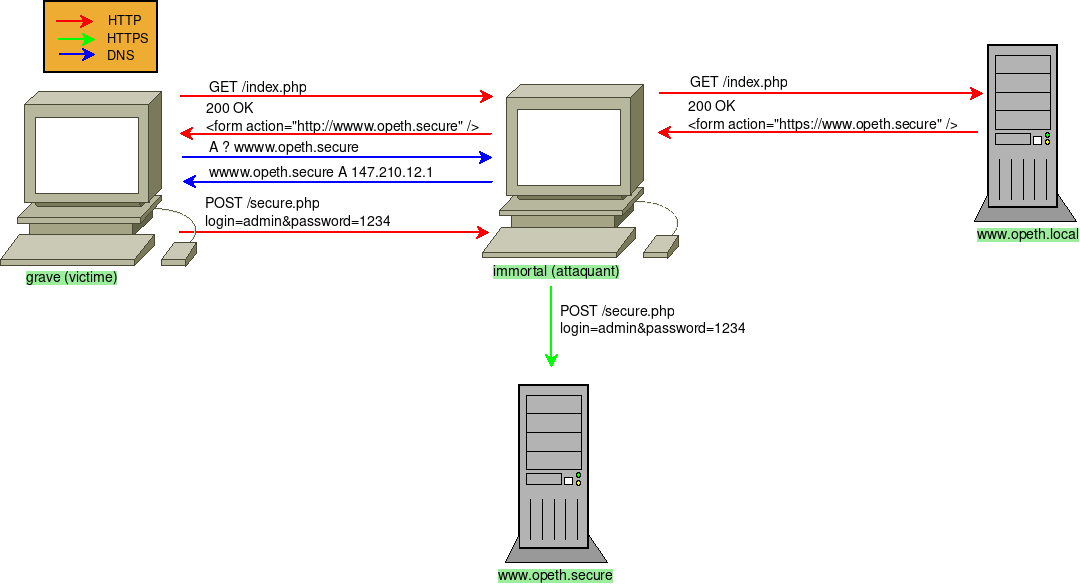
\includegraphics[width=\linewidth]{../medias/sslstrip2/attack.png}
\end{frame}
